\documentclass[9pt,twocolumn,twoside,]{pnas-new}

% Use the lineno option to display guide line numbers if required.
% Note that the use of elements such as single-column equations
% may affect the guide line number alignment.


\usepackage[T1]{fontenc}
\usepackage[utf8]{inputenc}

% tightlist command for lists without linebreak
\providecommand{\tightlist}{%
  \setlength{\itemsep}{0pt}\setlength{\parskip}{0pt}}


% Pandoc citation processing
\newlength{\cslhangindent}
\setlength{\cslhangindent}{1.5em}
\newlength{\csllabelwidth}
\setlength{\csllabelwidth}{3em}
\newlength{\cslentryspacingunit} % times entry-spacing
\setlength{\cslentryspacingunit}{\parskip}
% for Pandoc 2.8 to 2.10.1
\newenvironment{cslreferences}%
  {}%
  {\par}
% For Pandoc 2.11+
\newenvironment{CSLReferences}[2] % #1 hanging-ident, #2 entry spacing
 {% don't indent paragraphs
  \setlength{\parindent}{0pt}
  % turn on hanging indent if param 1 is 1
  \ifodd #1
  \let\oldpar\par
  \def\par{\hangindent=\cslhangindent\oldpar}
  \fi
  % set entry spacing
  \setlength{\parskip}{#2\cslentryspacingunit}
 }%
 {}
\usepackage{calc}
\newcommand{\CSLBlock}[1]{#1\hfill\break}
\newcommand{\CSLLeftMargin}[1]{\parbox[t]{\csllabelwidth}{#1}}
\newcommand{\CSLRightInline}[1]{\parbox[t]{\linewidth - \csllabelwidth}{#1}\break}
\newcommand{\CSLIndent}[1]{\hspace{\cslhangindent}#1}


\templatetype{pnasresearcharticle}  % Choose template

\title{Les scientifiques sont-ils crédibles ?}

\author[a,1]{Jordan Lenneville}

  \affil[a]{Université de Sherbrooke, Écologie, 2500 bd de l'Université,
Sherbrooke, Qc, J1K 2R1}


% Please give the surname of the lead author for the running footer
\leadauthor{Lenneville}

% Please add here a significance statement to explain the relevance of your work
\significancestatement{Cet article a été rédigé dans le cadre du cours
de Méthodes en écologie computationnelle (BIO500). Ce travail à comme
but de formuler et défendre une opinion sur les enjeux de
reproductibilité en écologie. Plus précisément, les élèves sont mendatés
à s'exprimer sur l'importance de la transparence et des standards de
reproductibilité dans un contexte où il y a une accélération de la
recherche.}


\authorcontributions{}



\correspondingauthor{\textsuperscript{1} E-mail:
\href{mailto:lenj0501@USherbrooke.ca}{\nolinkurl{lenj0501@USherbrooke.ca}}}

% Keywords are not mandatory, but authors are strongly encouraged to provide them. If provided, please include two to five keywords, separated by the pipe symbol, e.g:
 \keywords{  Reproductibilité |  Transparence |  true |  true |  true  } 

\begin{abstract}
résumé de 100 mots
\end{abstract}

\dates{This manuscript was compiled on \today}
\doi{\url{www.pnas.org/cgi/doi/10.1073/pnas.XXXXXXXXXX}}

\begin{document}

% Optional adjustment to line up main text (after abstract) of first page with line numbers, when using both lineno and twocolumn options.
% You should only change this length when you've finalised the article contents.
\verticaladjustment{-2pt}



\maketitle
\thispagestyle{firststyle}
\ifthenelse{\boolean{shortarticle}}{\ifthenelse{\boolean{singlecolumn}}{\abscontentformatted}{\abscontent}}{}

% If your first paragraph (i.e. with the \dropcap) contains a list environment (quote, quotation, theorem, definition, enumerate, itemize...), the line after the list may have some extra indentation. If this is the case, add \parshape=0 to the end of the list environment.

\acknow{Merci Dominique pour ce cours qui est utile pour optimiser notre
temps de codage. J'ai surtout aimer travailler avec Rmarkdown. Bon été!

\textbf{Bibliographie}}

\hypertarget{introduction}{%
\section*{Introduction}\label{introduction}}
\addcontentsline{toc}{section}{Introduction}

Introduction à la reproductibilité, transparence et parler un peu de
l'urgence de publié de ce temps-ci (1).

\hypertarget{argumentation}{%
\section*{Argumentation}\label{argumentation}}
\addcontentsline{toc}{section}{Argumentation}

\hypertarget{probluxe8mes}{%
\subsection*{Problèmes}\label{probluxe8mes}}
\addcontentsline{toc}{subsection}{Problèmes}

a

\hypertarget{solutions}{%
\subsection*{Solutions}\label{solutions}}
\addcontentsline{toc}{subsection}{Solutions}

b

\hypertarget{format}{%
\subsection*{Format}\label{format}}
\addcontentsline{toc}{subsection}{Format}

Many authors find it useful to organize their manuscripts with the
following order of sections; Title, Author Affiliation, Keywords,
Abstract, Significance Statement, Results, Discussion, Materials and
methods, Acknowledgments, and References. Other orders and headings are
permitted.

\begin{figure}
\centering

\includegraphics[width=0.5\textwidth,height=0.4\textheight]{grenouille.jpg}
\caption{Une belle gornouille qui danse}
\end{figure}

\begin{figure}
\centering
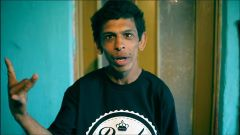
\includegraphics[width=0.5\textwidth,height=0.4\textheight]{Istadbut.jpg}
\caption{Jigoujigoula}
\end{figure}

\showmatmethods
\showacknow
\pnasbreak

\hypertarget{refs}{}
\begin{CSLReferences}{0}{0}
\leavevmode\vadjust pre{\hypertarget{ref-pennisi_spider_2020}{}}%
\CSLLeftMargin{1. }
\CSLRightInline{Pennisi E (2020) Spider biologist denies suspicions of
widespread data fraud in his animal personality research.
\emph{Science}.
doi:\href{https://doi.org/10.1126/science.abb1258}{10.1126/science.abb1258}.}

\end{CSLReferences}



% Bibliography
% \bibliography{pnas-sample}

\end{document}
